%!TEX program = xelatex
\documentclass[dvipsnames, svgnames,a4paper,11pt]{article}
% ----------------------------------------------------
%   中山大学物理与天文学院本科实验报告模板
%   作者:Huanyu Shi,2019级
%   知乎:https://www.zhihu.com/people/za-ran-zhu-fu-liu-xing
%   Github:https://github.com/Huanyu-Shi/SYSU-SPA-Labreport-Template
%   Last update : 2023.4.10
% ----------------------------------------------------

% ----------------------------------------------------- 
%	加边框的命令
%	参考:https://tex.stackexchange.com/questions/531559/how-to-add-the-page-border-for-first-two-pages-in-latex
\usepackage{tikz}
\usetikzlibrary{calc}
\usepackage{eso-pic}
\AddToShipoutPictureBG{%
\begin{tikzpicture}[overlay,remember picture]
\draw[line width=0.6pt] % 边框粗细
    ($ (current page.north west) + (0.6cm,-0.6cm) $)
    rectangle
    ($ (current page.south east) + (-0.6cm,0.6cm) $); % 边框位置
\end{tikzpicture}}


\usepackage{xcolor}
\definecolor{c1}{HTML}{2752C9} % 目录颜色
\definecolor{c2}{RGB}{190,20,83} % 引用颜色

\usepackage{ctex}
\usepackage[top=28mm,bottom=28mm,left=15mm,right=15mm]{geometry}
\usepackage{hyperref} 
\hypersetup{
	colorlinks,
	linktoc = section, % 超链接位置,选项有section, page, all
	linkcolor = c1, % linkcolor 目录颜色
	citecolor = c1  % citecolor 引用颜色
}
\usepackage{amsmath,enumerate,multirow,float}
\usepackage{tabularx}
\usepackage{tabu}
\usepackage{subfig}
\usepackage{fancyhdr}
\usepackage{graphicx}
\usepackage{wrapfig}  
\usepackage{physics}
\usepackage{appendix}
\usepackage{amsfonts}

%
\usepackage{tcolorbox}
\tcbuselibrary{skins,breakable}
\newtcolorbox{tbox}[2][]{
    colframe=black!70!,
    breakable,
    enhanced,
	boxrule =0.5pt,
    title = {#2},
    fonttitle = \large\kaishu\bfseries,
	drop fuzzy shadow,
    #1
}
\newtcolorbox[auto counter,number within=section]{question}[1][]{
  top=2pt,bottom=2pt,arc=1mm,
  boxrule=0.5pt,
%   frame hidden,
  breakable,
  enhanced, %跨页后不会显示下边框
  coltitle=c1!80!gray,
  colframe=c1,
  colback=c1!3!white,
  drop fuzzy shadow,
  title={思考题~\thetcbcounter:\quad},
  fonttitle=\bfseries,
  attach title to upper,
  #1
}
\newcommand{\setLhead}[1]{%
  \lhead{{\color{gray}\kaishu #1}} % 定义新的命令,设置右边页眉的内容
}
\newcommand{\setRhead}[1]{%
  \rhead{{\color{gray}\kaishu #1}} % 定义新的命令,设置右边页眉的内容
}
% ---------------------------------------------------------------------
%	利用cleveref改变引用格式,\cref是引用命令
\usepackage{cleveref}
\crefformat{figure}{#2{\textcolor{c2}{图 #1}}#3} % 图片的引用格式
\crefformat{equation}{#2{(\textcolor{c2}{#1})}#3} % 公式的引用格式
\crefformat{table}{#2{\textcolor{c2}{表 #1}}#3} % 表格的引用格式


% ---------------------------------------------------------------------
%	页眉页脚设置
\fancypagestyle{plain}{\pagestyle{fancy}}
\pagestyle{fancy}
\setLhead{中山大学物理与天文学院基础物理实验预习报告}
%\lhead{\kaishu 中山大学物理与天文学院物理实验\uppercase\expandafter{\romannumeral3}} % 左边页眉,学院 + 课程
%\rhead{{\color{gray}\kaishu Template 实验报告模板}} % 右边页眉,实验报告标题
\setRhead{实验1\hspace{1pt}冰的熔化热测量}
\cfoot{\thepage} % 页脚,中间添加页码


% ---------------------------------------------------------------------
%	对目录、章节标题的设置
\renewcommand{\contentsname}{\centerline{\huge 目录}}
\usepackage{titlesec}
\usepackage{titletoc}
% \titleformat{章节}[形状]{格式}{标题序号}{序号与标题间距}{标题前命令}[标题后命令]
\titleformat{\section}{\centering\LARGE\songti}{}{1em}{}

% ---------------------------------------------------------------------
%   listing代码环境设置
\usepackage{listings}
\lstloadlanguages{python}
\lstdefinestyle{pythonstyle}{
backgroundcolor=\color{gray!5},
language=python,
frameround=tftt,
frame=shadowbox, 
keepspaces=true,
breaklines,
columns=spaceflexible,                   
basicstyle=\ttfamily\small, % 基本文本设置,字体为teletype,大小为scriptsize
keywordstyle=[1]\color{c1}\bfseries, 
keywordstyle=[2]\color{Red!70!black},   
stringstyle=\color{Purple},       
showstringspaces=false,
commentstyle=\ttfamily\scriptsize\color{green!40!black},%注释文本设置,字体为sf,大小为smaller
tabsize=2,
morekeywords={as},
morekeywords=[2]{np, plt, sp},
numbers=left, % 代码行数
numberstyle=\it\tiny\color{gray}, % 代码行数的数字字体设置
stepnumber=1,
rulesepcolor=\color{gray!30!white}
}




% ---------------------------------------------------------------------
%	其他设置
\def\degree{${}^{\circ}$} % 角度
\graphicspath{{./images/}} % 插入图片的相对路径
\allowdisplaybreaks[4]  %允许公式跨页 % 导入模板的相关设置
\usepackage{lipsum}
\usepackage{indentfirst}
\usepackage{pdfpages}
\usepackage{multirow}
\usepackage{subfig}
\usepackage{graphicx}
\usepackage{float} 
\usepackage{booktabs}
\usepackage{enumerate}
\usepackage{makecell} 
\renewcommand{\d}{\mathrm{d}}
\newcommand{\upcite}[1]{\textsuperscript{\textsuperscript{\cite{#1}}}}


%---------------------------------------------------------------------
%	正文
%---------------------------------------------------------------------
\newcommand{\exname}{迈克尔逊干涉实验}%实验名称
\setRhead{\exname}
\begin{document}


\begin{table}
	\renewcommand\arraystretch{1.7}
	\begin{tabularx}{\textwidth}{
		|X|X|X|X
		|X|X|X|X|}
	\hline
	\multicolumn{2}{|c|}{预习报告}&\multicolumn{2}{|c|}{实验记录}&\multicolumn{2}{|c|}{分析讨论}&\multicolumn{2}{|c|}{总成绩}\\
	\hline
	 \hspace{0.625cm}25& & \hspace{0.625cm}30  & & \hspace{0.625cm}25  & &  \hspace{0.625cm}80 & \\
	\hline
	\end{tabularx}
\end{table}


\begin{table}
	\renewcommand\arraystretch{1.7}
	\begin{tabularx}{\textwidth}{|X|X|X|X|}
	\hline
	专业:& 物理学类 &年级:&2023级 \\
	\hline
	姓名:& 姚昊廷  & 学号:&22322091\\
	\hline
	日期:&2025.3.4 & 教师签名:& \\
	\hline
	\end{tabularx}
\end{table}

\begin{center}
	\LARGE \exname
\end{center}

\textbf{【实验报告注意事项】}
\begin{enumerate}
	\item 实验报告由三部分组成:
	\begin{enumerate}
		\item 预习报告:阅读\underline{\textbf{实验讲义}},弄清实验原理,了解实验需要测量的物理量,完成预习思考题。将预习报告带到实验室并在开始实验前由实验教师或助教检查。预习成绩低于10分(共20分)者不能做实验。
	    \item 实验记录:认真、客观记录实验条件、实验过程中的现象以及数据。实验记录请用珠笔或者钢笔书写并签名(\textcolor{red}{\textbf{用铅笔记录的被认为无效}})。\textcolor{red}{\textbf{保持原始记录,包括写错删除部分。}}离开前请实验教师或助教检查记录并签名。
	    \item 分析讨论:处理实验原始数据,对数据的可靠性和合理性进行分析;按规范呈现数据和结果;分析物理现象(含回答实验思考题,写出思考过程);最后得出结论。
	\end{enumerate}
	\item \underline{\textbf{实验报告}}就是将预习报告、实验记录、和数据处理与分析合起来,加上本页封面。实验记录须手写,预习报告和分析讨论部分手写或打印均可。
	\item 每次完成实验后的一周内交\textbf{实验报告}(特殊情况不能超过两周),每份报告必须注明姓名和学号,合作者和学号,否则按零分处理。
\end{enumerate}

\textbf{【安全注意事项】}
\begin{enumerate}
	\item 实验过程中,光源不要随意打开关闭;
	\item 严禁用手触光学镜头的表面;
	\item 严禁用强力和斜向力旋转测微头,这样会损坏测微头或其他部件;
	\item 不要拆卸传动机构,以免影响仪器正常使用;
	\item 实验过程中,数条纹时,避免桌面的振动。
\end{enumerate}


\clearpage
\tableofcontents
\clearpage

\setcounter{section}{0}
\section{\exname\ \textbf{预习报告}}
	
\subsection{实验目的}
\begin{enumerate}
	\item 了解迈克尔逊干涉仪的构造、原理和调节方法;
	\item 学习用迈克尔逊干涉仪测量单色光波长的方法;
	\item 学习用迈克尔逊干涉仪测量钠光谱波长差的方法;
	\item 观察等倾、等厚干涉现象及调节白光干涉条纹。
\end{enumerate}
\subsection{仪器用具}
\begin{table}[htbp]
	\centering
	\renewcommand\arraystretch{1.6}
	% \setlength{\tabcolsep}{10mm}
	\begin{tabular}{p{0.05\textwidth}|p{0.20\textwidth}|p{0.05\textwidth}|p{0.5\textwidth}}
	\hline
	编号& 仪器用具名称 & 数量 &  主要参数(型号,测量范围,测量精度等) \\
	\hline
	1&精密干涉仪&1 &SGM-4\\
	2&He-Ne激光器&1 &\\
	3&钠钨双灯&1 &\\
	4&汞灯&1 &\\
	5&透明薄片&1 &\\
	6&螺旋测微计&1 &\\
	\hline
\end{tabular}
\end{table}


\subsection{原理概述}
\begin{question}
	测量He-Ne激光波长
	\tcblower
	当激光束通过迈克尔逊干涉仪时,分束后分别经两臂反射后重新合束形成干涉条纹。若移动其中一面反射镜,镜子位移 \(\Delta d\) 会导致干涉条纹发生移动,其关系满足:
\[
2\Delta d = \Delta N\lambda\tag{1}
\]
其中,\(\Delta N\) 为条纹移动数目,\(\lambda\) 为激光波长。通过精确测量 \(\Delta d\) 与 \(\Delta N\),可计算出 \(\lambda\)。实验中采用非定域干涉条纹法测定激光波长。首先,按照参考书目原理概述中所述方法调出激光干涉圆条纹(等倾干涉);然后,单向缓慢旋转微调手轮以移动镜子 M2,直至干涉环中心达到最暗(或最亮)状态,此时记录 M2 的位置 \(d_1\)。接着,继续沿同一方向转动微调手轮,当条纹累计“吞进”或“吐出”的数目达到 \(\Delta N\) 时,再记录 M2 的位置 \(d_2\),设 M2 的位移变化为 \(\Delta d\)。根据双光束干涉原理,可利用这些数据计算激光的波长:
\[
\lambda = \frac{2\Delta d}{\Delta N}\tag{2}
\]
在测量过程中,累计条纹变化数目 \(\Delta N\) 不少于 500 条,建议每累计 50 条时读取一次数据,连续采集 10 组数据,并采用逐差法进行数据处理。
\end{question}

\begin{question}
	测钠双黄线的波长差
	\tcblower
	钠黄光含有两种波长相近的光(\(\lambda_1 = 589.0 \text{nm}\),\(\lambda_2 = 589.6 \text{nm}\))。采用钠灯作光源时,两条谱线形成各自的干涉条纹,在视场中的两套干涉条纹相互叠加。由于波长不同,同级条纹之间会产生错位(\(\lambda_1\)的某一级的暗条纹可能会和\(\lambda_2\)的另一级的亮条纹重合)。在移动反射镜M1(光程差发生变化)过程中,干涉条纹会出现清晰与模糊的周期性变化,称为“光拍现象”。其原理如下。
	\begin{figure}[H]
		\centering
		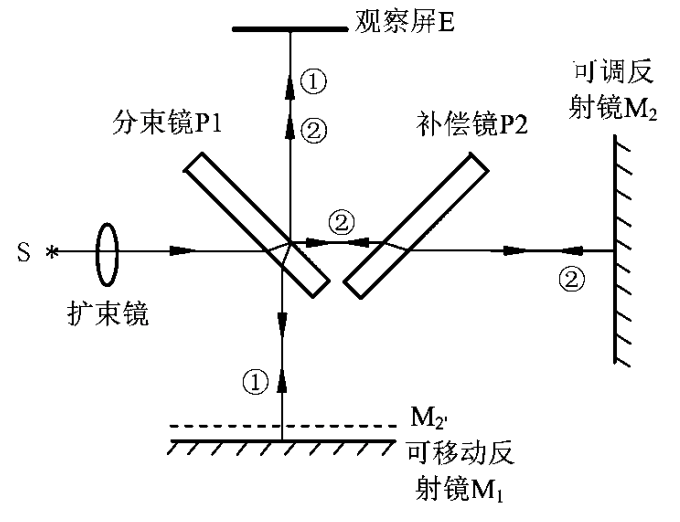
\includegraphics[width=0.5\textwidth]{迈克尔逊1.png}
		\caption{迈克尔逊干涉仪光路图}
	\end{figure}
	当M1与M2平行时,记M2的虚像M2'与M1之间的距离d,则两束光在观察屏(视场)E中心处的光程差为$L = 2d$。对波长为\(\lambda_1\)的入射光,由光的干涉条件可知:当\(L = k_1\lambda_1\)(\(k_1\)为整数)时,在视场E中心处干涉加强;对波长为\(\lambda_2\)的入射光,当\(L = \left(k_2 + \frac{1}{2}\right)\lambda_2\)(\(k_2\)为整数)时,在视场E中心处干涉减弱。

视场E中心处\(\lambda_1\)和\(\lambda_2\)两种单色干涉条纹相互叠加。若逐渐增大M1与M2'的间距d,当\(\lambda_1\)的第\(k_1\)级亮条纹和\(\lambda_2\)的第\(k_2\)级暗条纹相重合时(见图(二)A处),叠加而成的干涉条纹清晰度最低,此时干涉条纹出现第一次模糊,记录此时的光程差为\(L_A\),有

\[
L_A = k_1\lambda_1 = \left( k_2 + \frac{1}{2} \right) \lambda_2\tag{3}
\]

若继续增大M1与M2的间距,使得视场E中心处的光程差增加至\(L_B\),此时\(\lambda_1\)的第\(k_1 + n\)级亮条纹和\(\lambda_2\)的第\(k_2 + n\)级亮条纹相重合(见图(二)B处,图中\(n = 3\)),叠加而成的干涉条纹亮度最高,此时干涉条纹恢复清晰。继续增大M1与M2的间距,使得视场E中心处的光程差增加至\( L_c \),此时\(\lambda_1\)的第\(( k_1 + m )\)级亮条纹和\(\lambda_2\)的第\(( k_2 + m - 1 )\)级暗条纹相重合时(见图(二)C处,图中\( m = 5 \)),叠加而成的干涉条纹清晰度再次出现最低,此时干涉条纹出现第二次模糊,记录此时的光程差为\( L_c \),有
\[ 
L_c = \left( k_1 + m \right) \lambda_1 = \left[ k_2 + (m - 1) + \frac{1}{2} \right] \lambda_2 \tag{4} 
\]

设干涉条纹出现一次“模糊→清晰→模糊”的变化时,反射镜M1的移动距离为\(\Delta d\),

(4)式减(3)式可求得A处和C处前后的光程差变化为

\[ 
\Delta L_{CA} = L_c - L_A = 2\Delta d = m\lambda_1 = (m - 1)\lambda_2 \tag{5} 
\]

上式最后一个等式移项可得

\[ 
\lambda_2 - \lambda_1 = \frac{\lambda_2}{m} \tag{6} 
\]

(5)式倒数第二个等式移项得\(m = 2\Delta d/\lambda_1\),代入(6)式得

\[ 
\Delta \lambda \equiv \lambda_2 - \lambda_1 = \frac{\lambda_1\lambda_2}{2\Delta d} = \frac{\bar{\lambda}^2}{2\Delta d} \tag{7} 
\]

\(\bar{\lambda} = (\lambda_1 + \lambda_2)/2\)为钠双黄线波长的平均值。记录下干涉条纹出现一次“模糊→清晰→模糊”的变化时,反射镜M1移动的距离\(\Delta d\),结合钠双黄线的平均波长\(\bar{\lambda}\),即可利用(7)式求得钠双黄线的波长差\(\Delta \lambda\)。
	\begin{figure}[H]
		\centering
		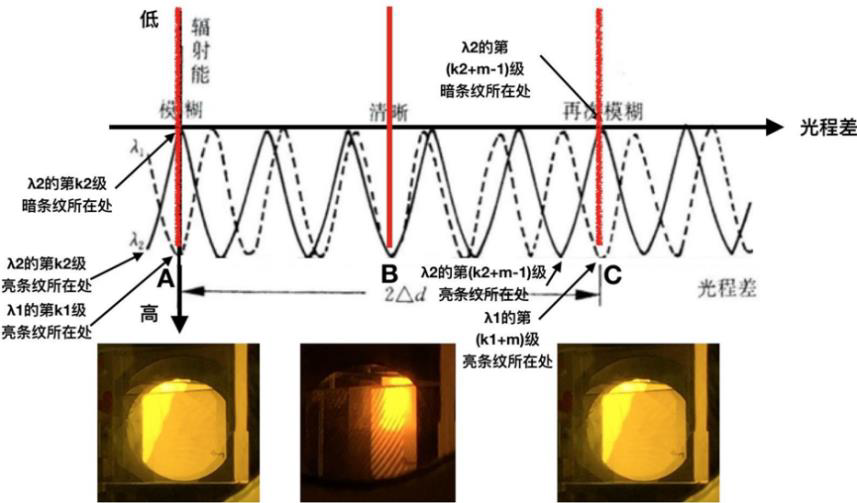
\includegraphics[width=0.5\textwidth]{迈克尔逊2.png}
		\caption{“光拍”现象及其原理}
	\end{figure}
\end{question}

\begin{question}
	白光干涉的调节,并测定透明薄片的厚度$t$或者折射率$n$
	\tcblower
	在迈克尔逊干涉实验中,如图(一)所示,先采用激光光源(安装上扩束镜),调节出定域等倾干涉圆环。再调节可移动反射镜M1的预置测微头,减小两干涉臂的光程差\(L\)(此过程中干涉圆环不断内缩,在观察屏中心E处不断“消失”),直至观察屏上只剩下几个较粗的干涉圆环(或圆环几乎消失,如图(三)所示)。这时候意味着两干涉臂的光程差\(L\)近似等于零。【提示:调节可移动反射镜M1的预置测微头的过程中,会出现干涉圆环中心偏离观察屏中心的现象,这是因为由于仪器制造工艺等原因,光束经分束镜P1分束后,不是严格地垂直入射到两反射镜的缘故。故反射镜M1的移动距离较大时,会出现干涉条纹跑偏的现象。这时可以轻微地调节反射镜M2背面的三个螺钉,使得干涉圆环的中心始终保持在观察屏E中心附近,如图(三)所示。】
	这时候撤掉扩束镜,换上扩散的汞灯光源(安装上毛玻璃),把观察屏翻到背后有玻璃的一面,然后微调可调反射镜M2背面的三个螺钉(调节M2的倾斜度),此时应能在玻璃镜(视场)中观察到域等倾干涉圆环。再调节可移动反射镜M1的预置测微头,减小两干涉臂的光程差\(L\)(此过程中干涉圆环不断内缩,在观察屏中心E处不断“消失”),直至观察屏上只剩下非常粗大的干涉圆环。
	换上扩散的白光光源(本实验中采用溴钨灯加毛玻璃代替),微调M2精密测微头,此时应能在玻璃镜(视场)中观察到彩色的条纹,此即为“白光等厚干涉条纹”。在视场中心处的彩色条纹之间还可观察到一条全黑的条纹,称为“中心暗纹”(如图(四)所示)。
	\begin{figure}[H]
		\centering
		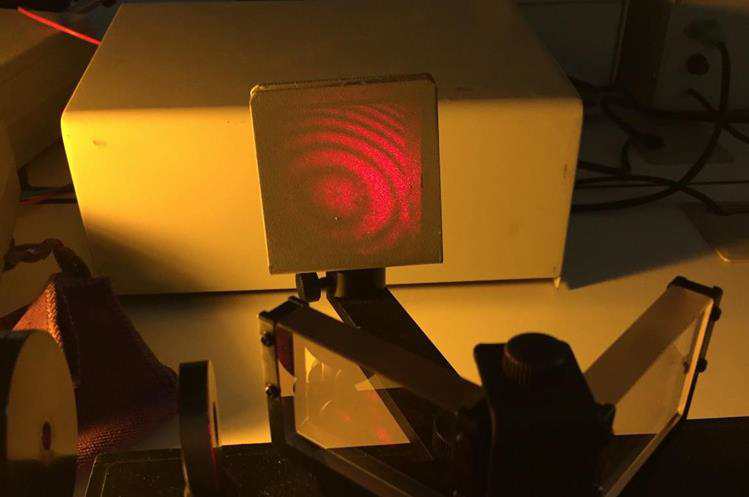
\includegraphics[width=0.5\textwidth]{迈克尔逊3.png}
		\caption{两干涉臂光程差几乎为零时,观察屏上只有少数几个等倾干涉圆环}
	\end{figure}
	\begin{figure}[H]
		\centering
		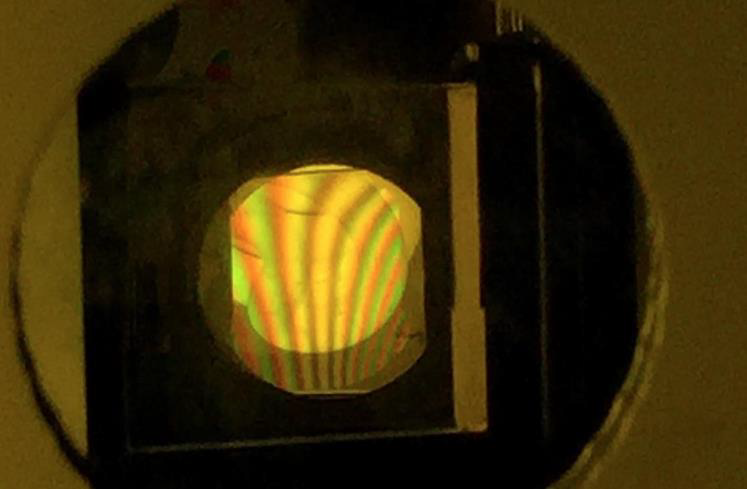
\includegraphics[width=0.5\textwidth]{迈克尔逊4.png}
		\caption{两干涉臂光程差几乎为零时,视场中的白光干涉的彩色条纹及其中心暗纹}
	\end{figure}
	然后在反射镜M1与分束镜P1之间放上折射率为\(n\),厚度为\(t\)的透明薄片,且尽量使薄片与M1镜平行,则此时两干涉臂的光程差要比原来增大

\[
\Delta L = 2t(n-1) \tag{8}
\]

放上透明薄片后,透过观察屏玻璃观察透明薄片处,可以看到视场中的白光干涉彩色
条纹消失。此时如果将反射镜M1镜(【注意:此时不能再动可调反射镜M2】)向前朝分束镜P1方向移动一段距离\(\Delta d\),使得\(\Delta d = \Delta L/2\)(此时候相当于虚光源 S1'和 S2'距离减小\(2\Delta d = \Delta L\),刚好是插入透明薄片后增加的光程差),则白光彩色干涉条纹重新出现(注意要调节反射镜M2镜的精密测微头,使得中心暗纹移到视场中央)。此时有

\[
\Delta d = t(n-1)\tag{9}
\]

测出M1镜的移动量\(\Delta d\),若已知透明薄片的厚度\(t\),则可由(9)式可求出透明薄片的折射率\(n\);反之,若已知透明薄片的折射率\(n\),可求出透明薄片的厚度\(t\)。
\end{question}
\subsection{预习思考题}
\begin{question}
    什么是光的相干性?怎样才能获得相干光?
	\tcblower
	光的相干性是指光波在时间和空间上保持稳定的相位关系,能够产生干涉现象的特性。相干性分为时间相干性(与光源单色性相关)和空间相干性(与光源尺寸相关)。获得相干光的
	方法有
	\begin{enumerate}
		\item 分波前法:将同一光源发出的光波分割为两部分
		\item 分振幅法:利用光学元件将一束光的振幅分为两部分
		\item 激光光源:激光具有高度的时间相干性(单色性好,和空间相干性(波前相位一致),可直接作为相干光源。
	\end{enumerate}
\end{question}

\begin{question}
    什么是“相干长度”和“相干时间”?如何计算光的相干长度和相干时间?
	\tcblower
	相干长度表示光波在传播方向上能保持相位相关性的最大空间距离。它反映了光源的时间相干性,单色性越好(频谱越窄),相干长度越长。
	相干时间表示光波保持相位相干性的时间范围。它与相干长度的关系为:
	\begin{align*}
	L_c = c \cdot \tau_c
	\end{align*}
	其中$c$为光速。
	计算方法为若已知光源的频谱线宽$\Delta \nu$,相干时间和相干长度可近似为:
	\begin{align*}
	\tau_c &\approx \frac{1}{\Delta \nu}, \\
	L_c &\approx \frac{c}{\Delta \nu}.
	\end{align*}
\end{question}

\begin{question}
    什么是非定域干涉?什么是定域干涉?什么是等倾干涉?什么是等厚干涉?
	\tcblower
	非定域干涉:干涉条纹出现在整个光场传播空间中,无需特定观察位置即可观察到清晰条纹。\\
	定域干涉:干涉条纹仅出现在特定空间区域(如薄膜表面附近),需在特定位置观察。\\
	等倾干涉:涉条纹由入射角相同的相干光形成,条纹形状为同心圆环。\\
	等厚干涉:干涉条纹由薄膜厚度相同的相干光形成,条纹形状反映厚度分布。
\end{question}

\begin{question}
    检索引力波探测器 LIGO 相关资料,简述引力波探测的原理。
	\tcblower
	LIGO由两臂垂直的干涉仪构成,激光被分束后分别在两臂中多次反射,最终合束产生干涉条纹。引力波引起的臂长差异会改变光程差,导致干涉条纹的亮度变化
	。当引力波经过时,一臂被压缩,另一臂被拉伸,导致两束激光的光程差变化。这种变化被转化为光子探测器接收的光强波动信号。
\end{question}
\clearpage
\setLhead{中山大学物理与天文学院基础物理实验记录}
\begin{table}
	\renewcommand\arraystretch{1.7}
	\centering
	\begin{tabularx}{\textwidth}{|X|X|X|X|}
	\hline
	专业:& 物理学类 &年级:& 2023级 \\
	\hline
	姓名: &姚昊廷& 学号:&22322091  \\
	\hline
	室温:&$22^\circ$C&实验地点:&A505  A4\\
	\hline
	学生签名:& & 评分: &\\
	\hline
	实验时间:& 2025.3.4& 教师签名:&\\
	\hline
	\end{tabularx}
\end{table}
\section{\exname\ \textbf{实验记录}}
\subsection{实验内容、步骤、结果}
\subsubsection{实验内容和步骤}
1.调节迈克尔逊干涉仪(He-Ne激光),使产生定域等倾干涉条纹
\begin{enumerate}
	\item 安装并打开He-Ne激光器(注意不要直射眼睛),但先不安装扩束镜,使激光 束从分束镜P1的中心附近入射;
	\item 调节可调反射镜M2背面的三个螺钉,使得M1和M2反射的光点的最亮处在 观察屏 E 上重合;
	\item 装上扩束镜(以获得点光源),此时应能在观察屏上看到等倾干涉条纹(如观 察不到,则可微调固定激光器的螺钉,使得光束能顺利通过扩束镜);
	\item 单向缓慢旋转精密测微头,移动镜子M2,直至干涉环中心达到最暗(或最亮)状态,此时记录M2的位置$d_1$。接着,继续沿同一方向转动精密测微头,当条纹累计“吞进” 或“ 吐出”的数目达到N时,再记录M2的位置$d_2$,设M2的位移变化为$\Delta d$;
	\item 根据(2)式计算He-Ne激光波长【提示:累计条纹变化数目N不少于500条,建议每累计50条时读取一次数据,连续采集10组数据,并采用逐差法进行数据处理】。
\end{enumerate}
记录结果如下:
\begin{table}[H]
	\centering
	\caption{测量He-Ne激光波长}
	\begin{tabular}{cc}
		\toprule
		$N$&$d_2$(mm)\\
		\midrule
		0&10.860\\
		50&11.472\\
		100&12.109\\
		150&12.733\\
		200&13.365\\
		250&13.433\\
		300&14.059\\
		350&14.690\\
		400&15.319\\
		450&15.960\\
		500&16.588\\
		\toprule
	\end{tabular}
\end{table}
2.测量钠双黄线的波长差
\begin{enumerate}
	\item 调节可移动反射镜M1的精密测微头,减小两干涉臂的光程差 L(此过程中干涉圆环不断内缩,在观察屏中心E处不断“消失”),直至观察屏上只剩下几个较粗的干涉圆环(或圆环几乎消失,如图(三)所示)。这时候两干涉臂的光程几乎相等,光程差近似等于零。【提示:调节可移动反射镜M1的精密测微头的过程中,会出现干涉圆环中心偏离观察屏中心的现象,这是因为由于仪器制造工艺等原因,光束经分束镜
	P1分束后,不是严格地垂直入射到两反射镜的缘故。故反射镜M1的移动距离较大时,会出现干涉条纹跑偏的现象。这时候可以轻微地调节反射镜M2背面的三个螺钉,使得干涉圆环的中心始终保持在观察屏E中心附近,如图(三)所示】;
	\item 不安装扩束镜。改用钠灯,灯前装有毛玻璃使光散射。观察屏改为平面玻璃反射镜;
	\item 从观察屏的玻璃中观察,仔细调节M2镜后的三颗倾斜度调节螺钉和M1镜的位置,可观察到黄黑相间的直线状的等厚干涉条纹;
	\item 调节精密测微头,移动反射镜M1,观察条纹“模糊→清晰→模糊”的周期变化过程,记录每一次干涉条纹“模糊”时候精密测微头的读数,随后计算出M1镜移动的距离$\Delta d$;
	\item 根据(7)式计算钠双黄线的波长差
\end{enumerate}
记录结果如下:
\begin{table}[H]
	\centering
	\caption{测量钠双黄线的波长差}
	\begin{tabular}{cccc}
		\toprule
		\multicolumn{2}{c}{第一次测量}&\multicolumn{2}{c}{第二次测量}\\
		\midrule
		模糊&21.121mm&模糊&21.103mm\\
		清晰&28.058mm&清晰&28.013mm\\
		模糊&35.010mm&模糊&34,983mm\\
		\toprule
	\end{tabular}
\end{table}
3.调节迈克尔逊白光干涉仪
\begin{enumerate}
	\item 重复步骤1和步骤2的(1),用He-Ne激光作为光源,调出等倾干涉圆环。调节预置测微头移动反射镜M2,使条纹变宽变稀,至观察屏上只有少数几个圆环,至此两干涉臂的光程几乎相等;
	\item 撤掉扩束镜,换上扩散的汞灯光源(毛玻璃),把观察屏翻到背后有玻璃的一面,然后微调可调反射镜M2背面的三个螺钉(调节M2的倾斜度),此时应能在玻璃镜(视场)中观察到域等倾干涉圆环。再调节可移动反射镜M1的预置测微头,减小两干涉臂的光程差L,直至观察屏上只剩下非常粗大的干涉圆环;
	\item 换上扩散的白光光源(本实验中采用溴钨灯加毛玻璃代替),微调M2精密测微头,此时应能在玻璃镜(视场)中观察到彩色的条纹,此即为“白光等厚干涉条纹”。彩色条纹之间还可观察到一条全黑的条纹,称为“中心暗纹”;
	\item 如实详细记录实验现象。
\end{enumerate}
\begin{figure}[H]
	\centering
	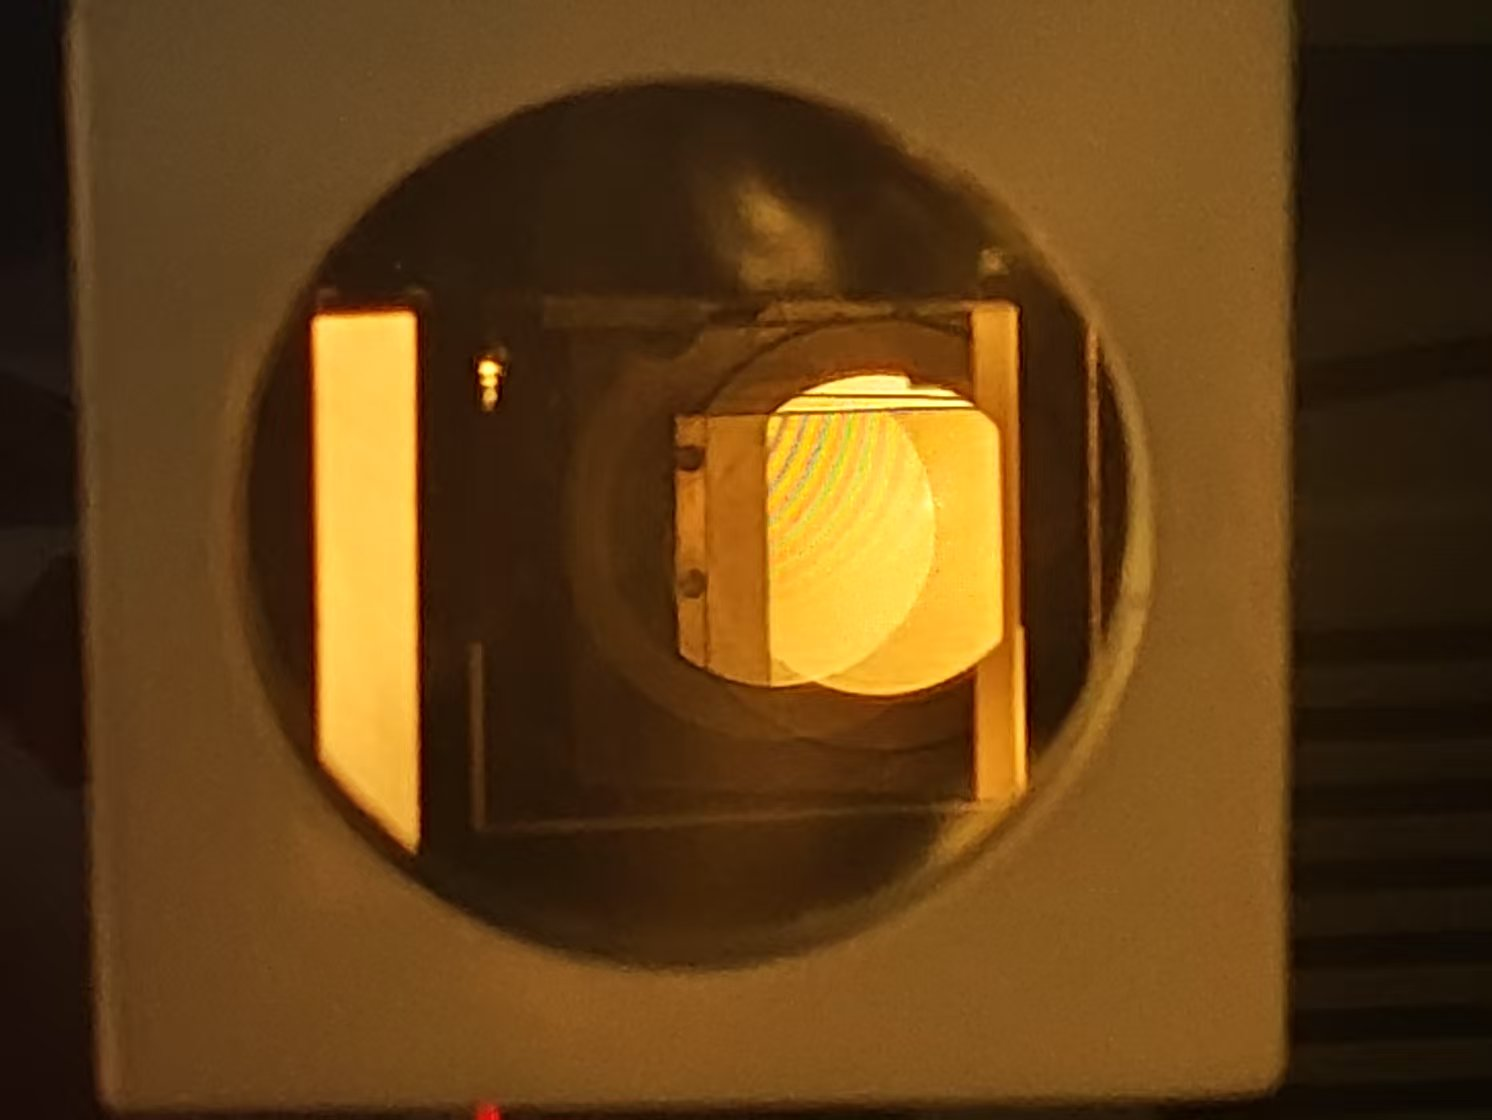
\includegraphics[width=\textwidth]{迈克尔逊白光干涉.jpg}
	\caption{迈克尔逊白光干涉}
\end{figure}
\subsection{实验过程遇到问题记录}
\begin{enumerate}
	\item 黄光干涉中模糊清晰判定过于不清晰
	\item 干涉仪平动与转动耦合过强,难以调节至只剩一个大光斑的情况。
\end{enumerate}

\clearpage
\setLhead{中山大学物理与天文学院基础物理实验分析与讨论}
\begin{table}
	\renewcommand\arraystretch{1.7}
	\begin{tabularx}{\textwidth}{|X|X|X|X|}
	\hline
	专业:& 物理学 &年级:& 2023级\\
	\hline
	姓名: &姚昊廷& 学号:&22322091 \\
	\hline
    日期:&2025.3.4 &  &\\
	\hline
	评分:&&教师签名:&\\
	\hline
	\end{tabularx}
\end{table}

\section{\exname\ \textbf{分析与讨论}}
\subsection{分析与讨论}
1.测量He-Ne激光波长
\begin{align*}
	\Delta d_1&=d_6-d_1=3.199\text{mm}\\
	\Delta d_2&=d_7-d_2=3.218\text{mm}\\
	\Delta d_3&=d_8-d_3=3.210\text{mm}\\
	\Delta d_4&=d_9-d_4=3.227\text{mm}\\
	\Delta d_5&=d_10-d_5=3.155\text{mm}\\
\end{align*}
故
\begin{align*}
	\overline{\Delta d}=\frac{\sum \Delta d_i}{5\times 5}=0.640\text{mm}
\end{align*}
测得波长为
\begin{align*}
	\lambda=\frac{2\overline{\Delta d}}{500\times 40}=640\text{nm}
\end{align*}
相对误差为
\begin{align*}
	\frac{640-633}{633}=1.1\%
\end{align*}
2.测量钠双黄线的波长差
\begin{align*}
	\overline{\Delta d}=\frac{\sum \Delta d_i}{2}=13.68\text{mm}
\end{align*}
测得波长差为
\begin{align*}
	\Delta \lambda=\frac{\overline{\lambda}^2}{2\overline{\Delta d}}=0.1\text{nm}
\end{align*}
相对误差为
\begin{align*}
	\frac{0.1-0.3}{0.3}=-66.7\%
\end{align*}
误差过大原因可能有
\begin{enumerate}
	\item 黄光干涉中模糊清晰判定过于不清晰
	\item 实验组数太少
\end{enumerate}
\subsection{实验后思考题}
\begin{question}
	迈克尔逊干涉仪观察到干涉条纹的条件是什么?激光干涉与白光干涉有哪些不同之处?
	\tcblower
	两干涉臂长差小于一半的相干长度,激光频谱较窄,相干长度长,相干性好,使得干涉容易发生。白光频谱较宽,相干长度短,导致干涉难以发生。
\end{question}

\begin{question}
	利用迈克尔逊激光干涉仪测量He-Ne激光波长的误差有哪些?如何减小误差?
	\tcblower
	主要误差来源:
	\begin{enumerate}
		\item 环境因素\begin{enumerate}
			\item 温度与气流:温度波动或空气流动引起空气折射率变化,导致光程差测量偏差。
			\item 振动:外界振动导致干涉条纹抖动,影响条纹计数准确性。
		\end{enumerate}
		\item 机械系统误差\begin{enumerate}
			\item 空程差:移动反射镜的螺杆存在回程间隙,导致位移测量不准确。
			\item 读数装置精度:螺旋测微器或位移传感器分辨率不足,引入位移测量误差。
		\end{enumerate}
		\item 人为误差\begin{enumerate}
			\item 条纹计数错误:手动计数时漏数或多数干涉条纹。
			\item 光路校准偏差:分束器或反射镜未严格垂直,导致非等倾干涉。
		\end{enumerate}
		\item 光源稳定性\begin{enumerate}
			\item 激光波长漂移:He-Ne激光器未充分预热或受温度影响,导致波长不稳定。
			\item 模式跳变:激光器多纵模运行导致干涉条纹对比度下降。
		\end{enumerate}
	\end{enumerate}
	减小误差方法:
	\begin{enumerate}
		\item 控制实验环境:在恒温、无气流(如封闭光路)和低振动环境(如光学隔振平台)中进行实验。
		\item 优化机械系统\begin{enumerate}
			\item 消除空程差:单向旋转螺杆测量位移,避免回程操作。
			\item 提高读数精度:使用高分辨率位移传感器(如激光干涉仪或压电陶瓷驱动器)。
		\end{enumerate}
		\item 稳定光源\begin{enumerate}
			\item 预热激光器30分钟以上,确保波长稳定。
			\item 使用单纵模He-Ne激光器,避免模式跳变影响条纹对比度。
		\end{enumerate}
		\item 自动化与校准\begin{enumerate}
			\item 自动条纹计数:采用光电探测器配合计数器,减少人为误差。
			\item 严格校准光路:调节反射镜使两束光严格垂直,获得清晰的等倾干涉圆环。
		\end{enumerate}
	\end{enumerate}
\end{question}

\begin{question}
	迈克尔逊干涉仪测量钠黄双线的误差有哪些?如何减小误差?
	\tcblower
	主要误差来源:
	\begin{enumerate}
		\item 钠黄双线本身的特性\begin{enumerate}
			\item 条纹对比度周期性变化:钠黄双线波长差导致干涉条纹对比度随光程差周期性变化(拍频现象),若未合理选择光程差范围,可能导致条纹模糊或计数错误。
			\item 非单色性误差:双线光谱宽度和间隔会使条纹位置偏移,影响波长计算精度。
		\end{enumerate}
		\item 光源稳定性不足\begin{enumerate}
			\item 钠灯预热不充分:钠灯需要较长时间(约15-30分钟)稳定,否则波长和强度波动。
			\item 电流波动:供电不稳导致钠灯发光波长漂移或闪烁,干扰条纹观测。
		\end{enumerate}
		\item 光程差控制误差\begin{enumerate}
			\item 超出相干长度:钠光的相干长度较短(约几毫米),若两臂光程差超过相干长度,条纹消失或对比度极低。
			\item 移动速度过快:手动移动反射镜时速度不均,导致漏数条纹或误判对比度变化周期。
		\end{enumerate}
		\item 人为观测误差:对比度极值误判:双线导致的条纹对比度周期性变化(如每移动一定距离出现一次“清晰-模糊-清晰”),若未准确记录极值点,会导致光程差计算错误。
	\end{enumerate}
	减小误差方法:
	\begin{enumerate}
		\item 针对性优化光程差范围:控制光程差在钠光相干长度内(约数毫米),确保条纹可见。
		\item 光源稳定性控制\begin{enumerate}
			\item 充分预热钠灯至稳定工作状态(30分钟以上)。
			\item 使用稳压电源减少电流波动,或选择高稳定性钠灯。
		\end{enumerate}
		\item 改进测量与计数方法\begin{enumerate}
			\item 半自动化计数:用光电探测器记录光强变化,结合示波器观察周期性信号,替代肉眼判断对比度变化。
			\item 多次重复测量:对同一光程差范围进行3-5次重复测量,取平均值减少随机误差。
		\end{enumerate}
	\end{enumerate}
\end{question}

\begin{question}
	如果利用迈克尔逊干涉仪测量透明薄片折射率,用激光干涉还是白光干涉好?为什么?
	\tcblower
	在使用迈克尔逊干涉仪测量透明薄片的折射率时,白光干涉比激光干涉更优,原因如下:
	\begin{enumerate}
		\item 白光的相干长度极短(通常仅几微米),干涉条纹仅在两臂光程差接近零时出现(即“零级条纹”)。插入透明薄片后,通过移动参考臂补偿光程差,使零级条纹重新出现。补偿距离直接对应薄片引入的光程差,无需依赖条纹移动计数,避免了激光干涉中因条纹周期性模糊导致的误差。
		\item 透明薄片折射率$n$与厚度$d$的关系为:
		\begin{align*}
			\Delta L=2d(n-1)
		\end{align*}
		白光干涉通过补偿距离$\Delta L$直接求解$n$,而激光干涉需通过条纹移动数$N$计算:
		\begin{align*}
			N=\frac{2d(n-1)}{\lambda}
		\end{align*}
		若薄片厚度$d$未知,激光法需额外测量$d$,而白光法可结合厚度测量(如机械测量)直接解算$n$,减少误差传递。
		\item 消除多值性问题
		激光干涉中,若光程差超过一个波长(即$N$为整数倍),条纹会周期性重复,导致$N$的计数歧义(例如 $N=10$ 和
		$N=11$ 可能难以区分)。白光干涉通过零级条纹的唯一性,彻底规避此问题。
	\end{enumerate}
\end{question}
\clearpage
% ---------------------------------------------------------------------
%   参考文献
%   注:使用参考文献时应按照xelatex->bibtex->xelatex->xelatex顺序进行编译
%\phantomsection
%\addcontentsline{toc}{section}{参考文献}
%\bibliographystyle{unsrt}
%\bibliography{myref}
%\begin{thebibliography}{9}
%	\bibitem{ref1} 沈雨欣,翁存程,蒋丽钦.双棱镜干涉法准确测量钠光波长[J].大学物理实验,2023,36(03):40-43.DOI:10.14139/j.cnki.cn22-1228.2023.03.008.
%	\bibitem{ref2} 牟泉润,孙丽媛,杜月棋,等.基于干涉原理的光波长测量装置设计[J].大学物理实验,2021,34(06):80-83+89.DOI:10.14139/j.cnki.cn22-1228.2021.06.018.
%	\bibitem{ref3} 王仁洲,杨涛.一种用激光干涉测量光波波长的新方法[J].大学物理实验,2014,27(06):41-43.DOI:10.14139/j.cnki.cn22-1228.2014.06.014.
%\end{thebibliography}


%\clearpage
\appendix
\appendixpage
\addappheadtotoc
%\subsection*{相图代码}
%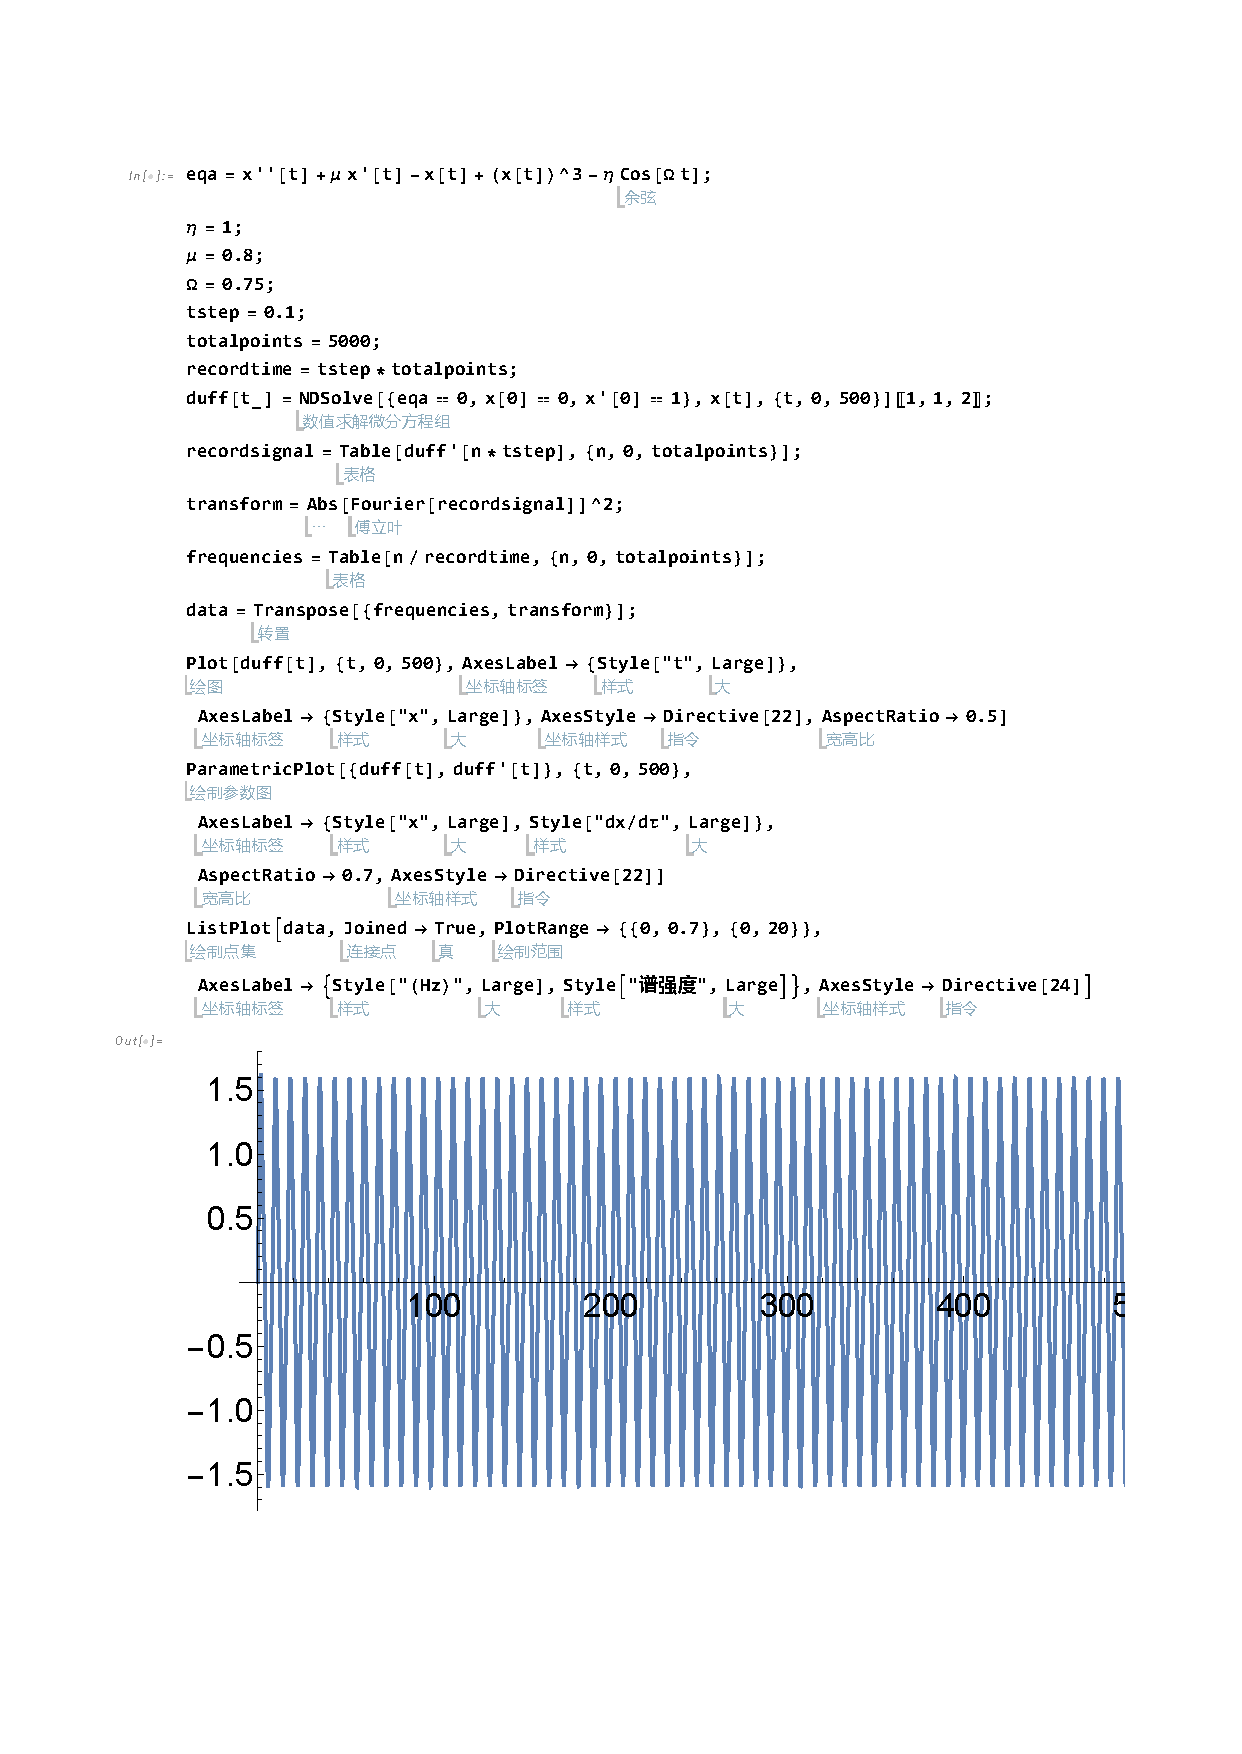
\includepdf[pages=-]{chaos.pdf}
\subsection*{原件}
%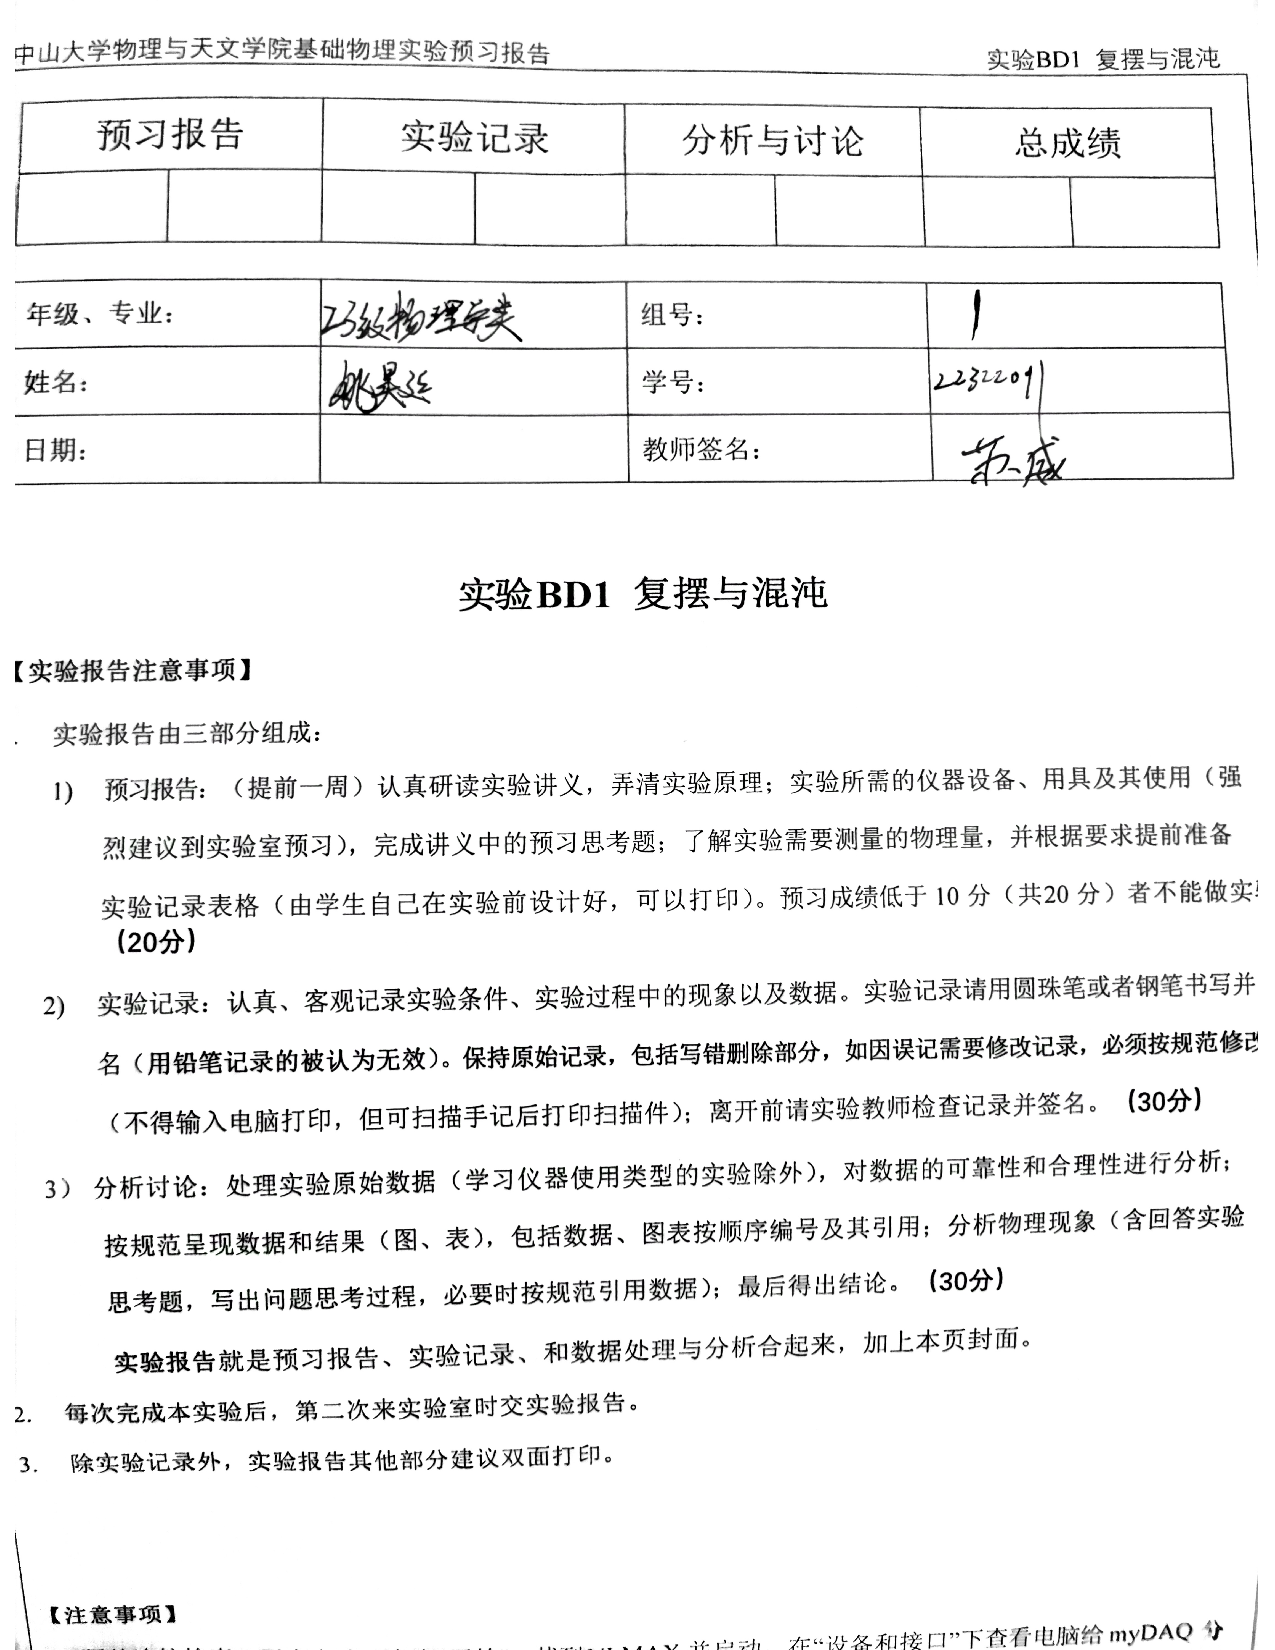
\includepdf[pages=-]{实验3原件.pdf}
%\begin{figure}[H]
%	\centering
%	\includegraphics[width=\textwidth]{焦距数据.jpg}
	
%\end{figure}
%\begin{figure}[H]
%	\centering
%	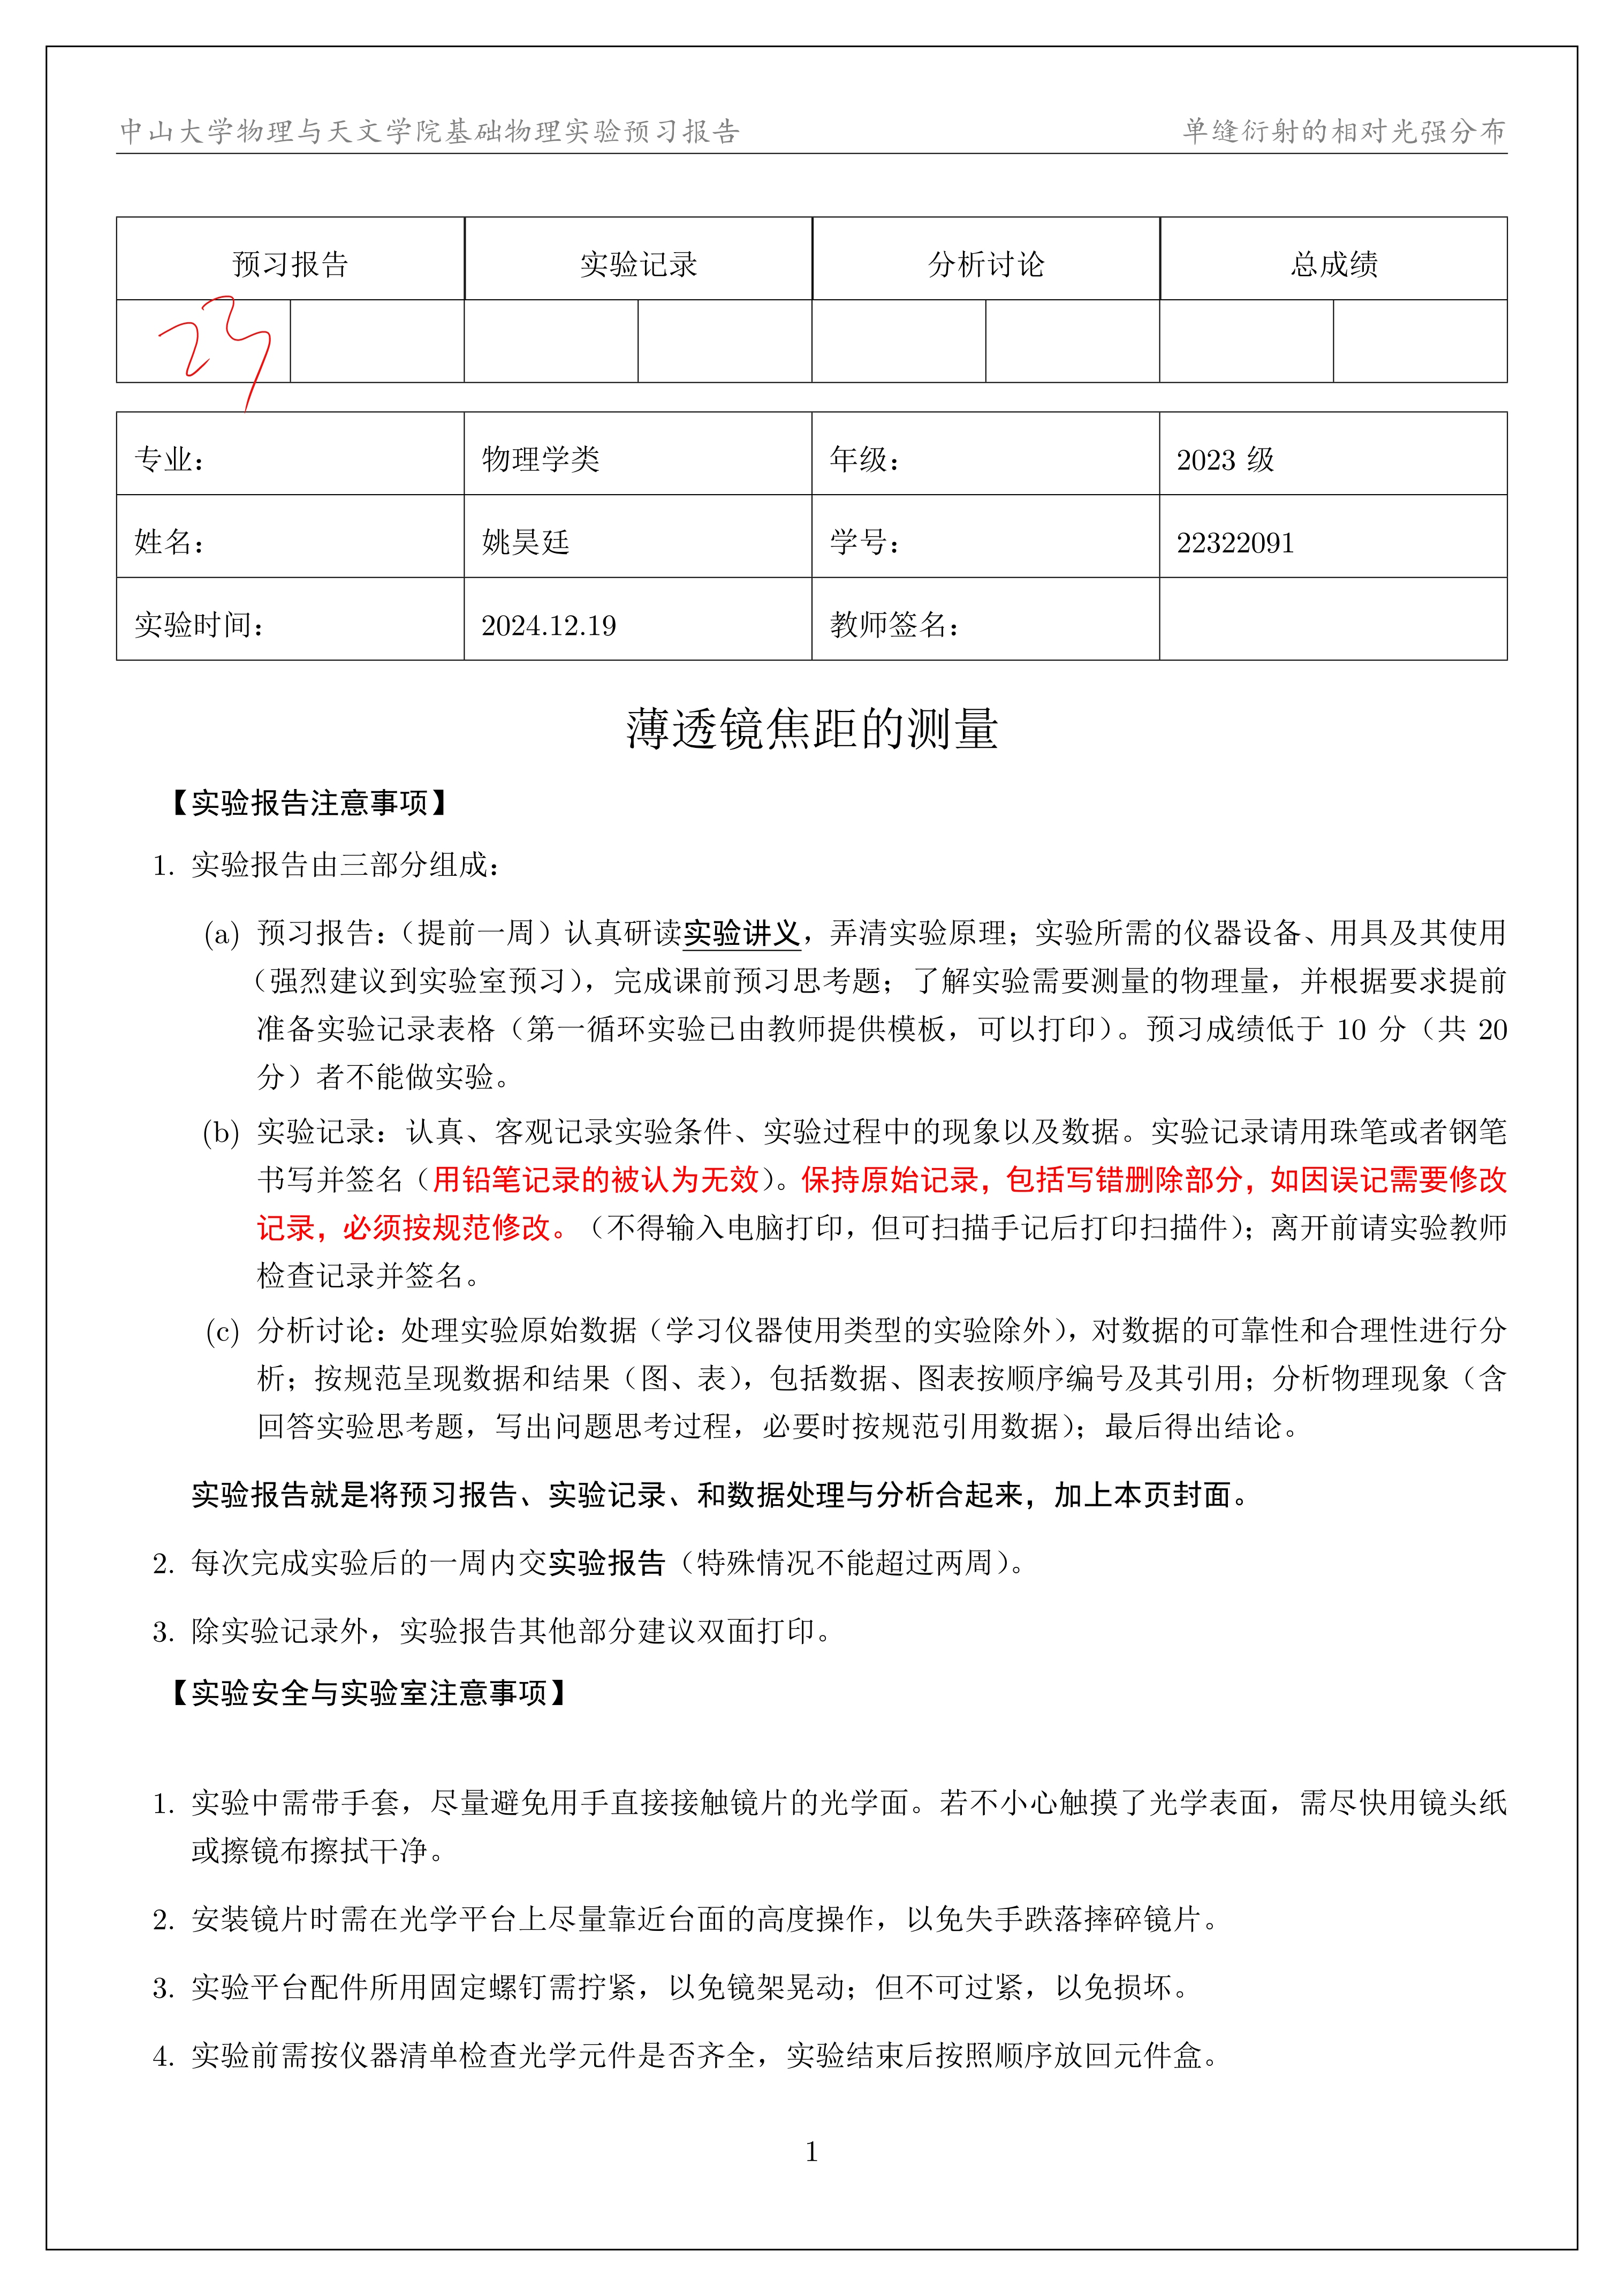
\includegraphics[width=\textwidth]{透镜焦距.jpg}
	
%\end{figure}

\begin{figure}[H]
	\centering
	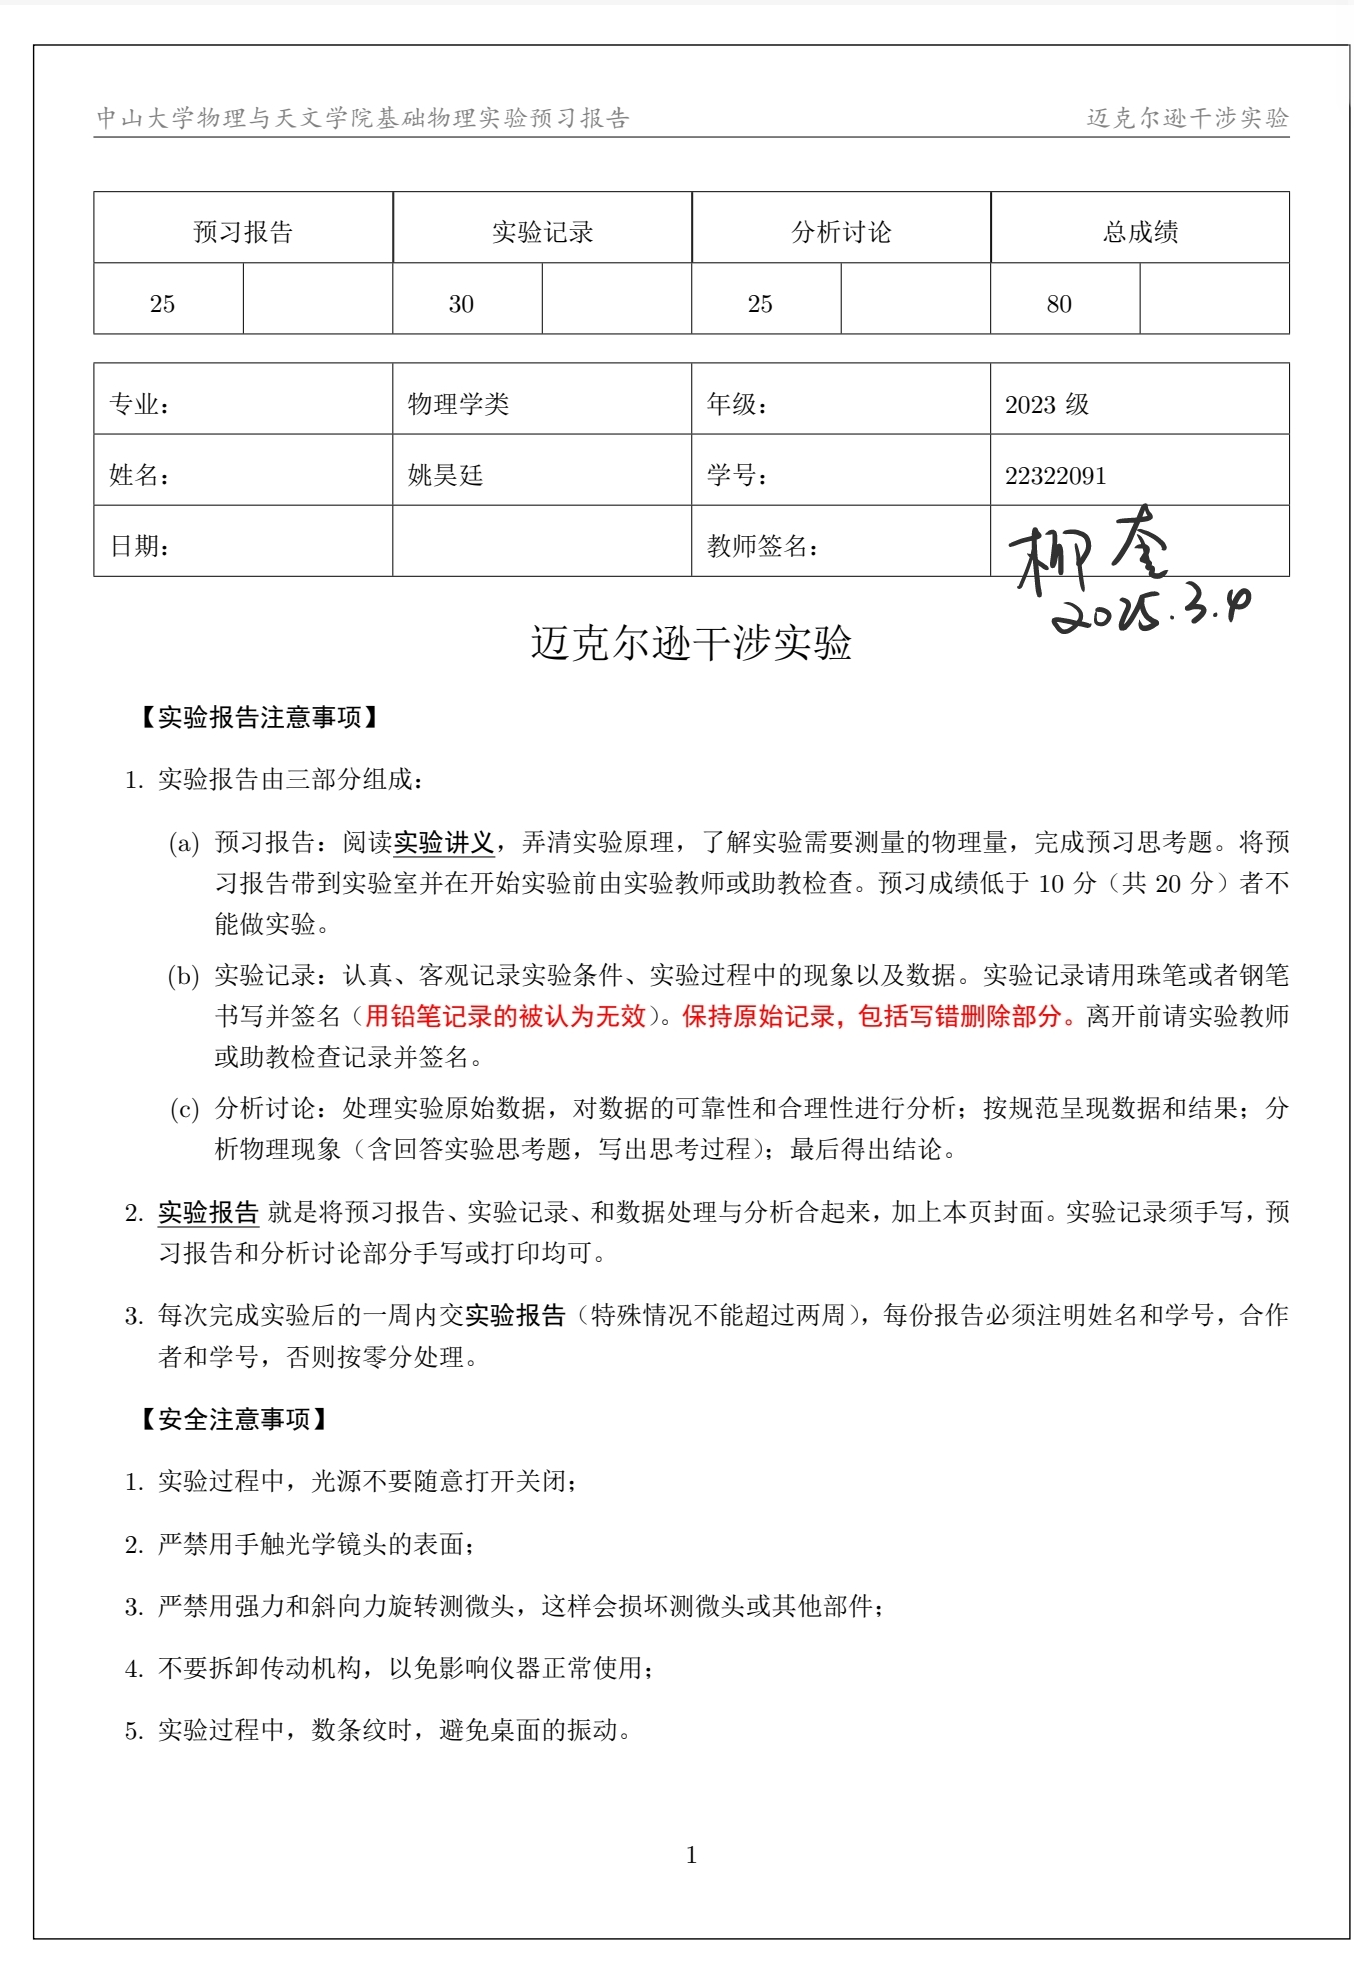
\includegraphics[width=0.4\textwidth]{迈克尔逊原件1.jpg}
	\includegraphics[width=0.4\textwidth]{迈克尔逊原件2.jpg}
%	\includegraphics[width=0.4\textwidth]{单缝原件3.jpg}
%	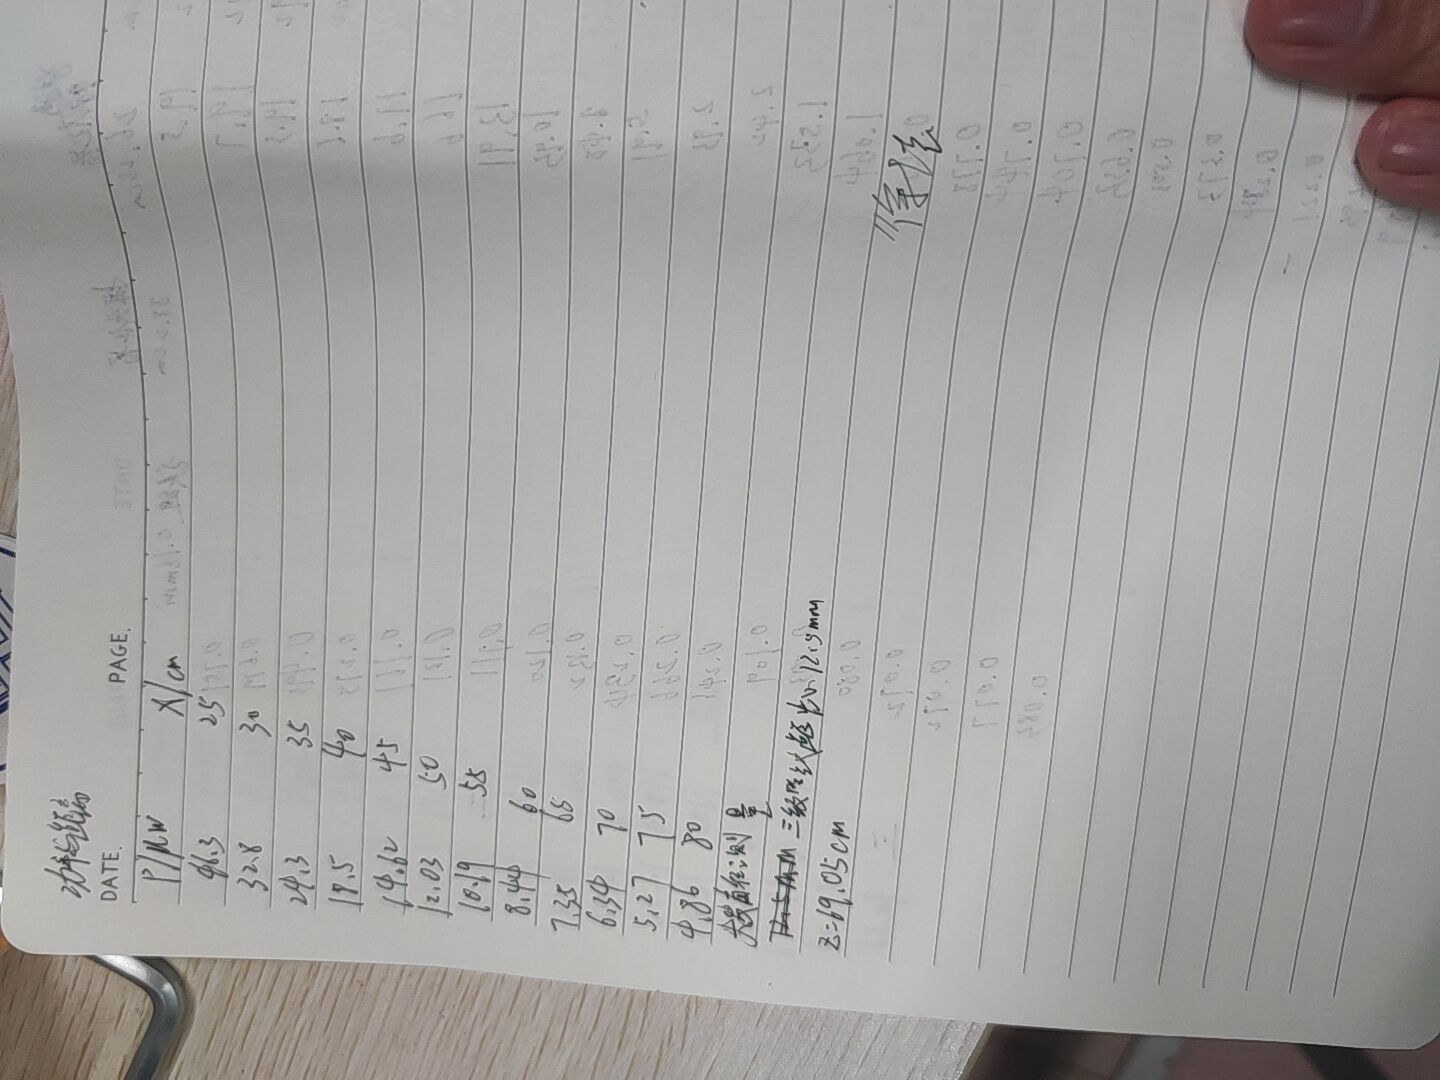
\includegraphics[width=0.4\textwidth]{单缝原件4.jpg}
\end{figure}
\subsection*{桌面}
\begin{figure}[H]
	\includegraphics[width=0.95\textwidth]{迈克尔逊桌面.jpg}
\end{figure}
\end{document}
%